%        File: Stanford_Machine_Learning_Notes.tex
%     Created: Mon May 18 11:00 pm 2020 E
% Last Change: Mon May 18 11:00 pm 2020 E
%
\documentclass[letter]{article}
\newcommand*{\vertbar}{\rule[-1ex]{0.5pt}{2.5ex}} % for complicated matrices
\newcommand*{\horzbar}{\rule[.5ex]{2.5ex}{0.5pt}}
\title{%
    Machine Learning\\
    \large Stanford University \\
    Professor Andrew Ng}

\author{Jordan Hong}
\date{\today}
\usepackage{graphicx}
\usepackage{amsfonts}
\usepackage{caption}
\usepackage{subcaption}
%\usepackage{color}   %May be necessary if you want to color links
\usepackage{hyperref}
\hypersetup{
    linktoc=all,     %set to all if you want both sections and subsections linked
}
\usepackage{amsmath}
\usepackage{listings}
\usepackage{color} %red, green, blue, yellow, cyan, magenta, black, white
\usepackage[T1]{fontenc}
% macro to select a scaled-down version of Bera Mono (for instance)
\makeatletter
\newcommand\BeraMonottfamily{%
  \def\fvm@Scale{0.85}% scales the font down
  \fontfamily{fvm}\selectfont% selects the Bera Mono font
}
\makeatother

\definecolor{mygreen}{RGB}{28,172,0} % color values Red, Green, Blue
\definecolor{mylilas}{RGB}{170,55,241}
\lstset{language=Matlab,%
    basicstyle=\BeraMonottfamily,
    breaklines=true,%
    frame=single,%
    morekeywords={matlab2tikz},%
    keywordstyle=\color{blue},%
    morekeywords=[2]{1}, keywordstyle=[2]{\color{black}},%
    identifierstyle=\color{black},%
    stringstyle=\color{mylilas},%
    commentstyle=\color{mygreen},%
    showstringspaces=false,%without this there will be a symbol in the places where there is a space
    emph=[1]{for,end,break},emphstyle=[1]\color{red}, %some words to emphasise
    %emph=[2]{word1,word2}, emphstyle=[2]{style},    
    gobble=8,%
    tabsize=4
}





\begin{document}
\maketitle
\tableofcontents
\newpage
    \section{Introduction}
    \subsection{What is Machine Learning}
    
    \begin{enumerate}
        \item Machine Learning 
            \begin{itemize}
                \item Grew out of work in Artificial Intelligence (AI)
                \item New capabilities for computers
            \end{itemize}
        \item Examples: 
            \begin{itemize}
                \item database mining
                \item applications can't programby hand (handwriting recognition, Natural Language Processing (NLP), Computer Vision) 
                \item Neuromorphic applications
            \end{itemize}
           
        \item Definition
            \begin{itemize}
                \item Arthur Samuel(1959) \\
                    \begin{quote}
                        Machine Learning: Field of study that gives computers the ability to learn without being explicitly programmed.

                    \end{quote}
                \item Tom Mitchell(1998) \\
                    \begin{quote}
                         Well-posed Learning Problem: A computer program is said to learn from experience E with respect to some task T and some performance measure P, if its performance on T, as measured by P, improves with experience E. 

                    \end{quote}
           \end{itemize}
        \item Machine Learning in this course:
            \begin{enumerate}
                \item Suupervised Learning
                \item Unsupervised Learning
                \item Others: reinforcement learning, recommender systems
                \item Practical application techniques
            \end{enumerate}
    \end{enumerate}

    
    \subsection{Supervised Learning}

        In supervised learning, the \emph{the right answer} is given. For example:
        \begin{enumerate}
            \item Regression: predict real-valued output.
            \item Classification: predict discrete-valued output.
        \end{enumerate}

    \begin{figure}[h]
        \centering
        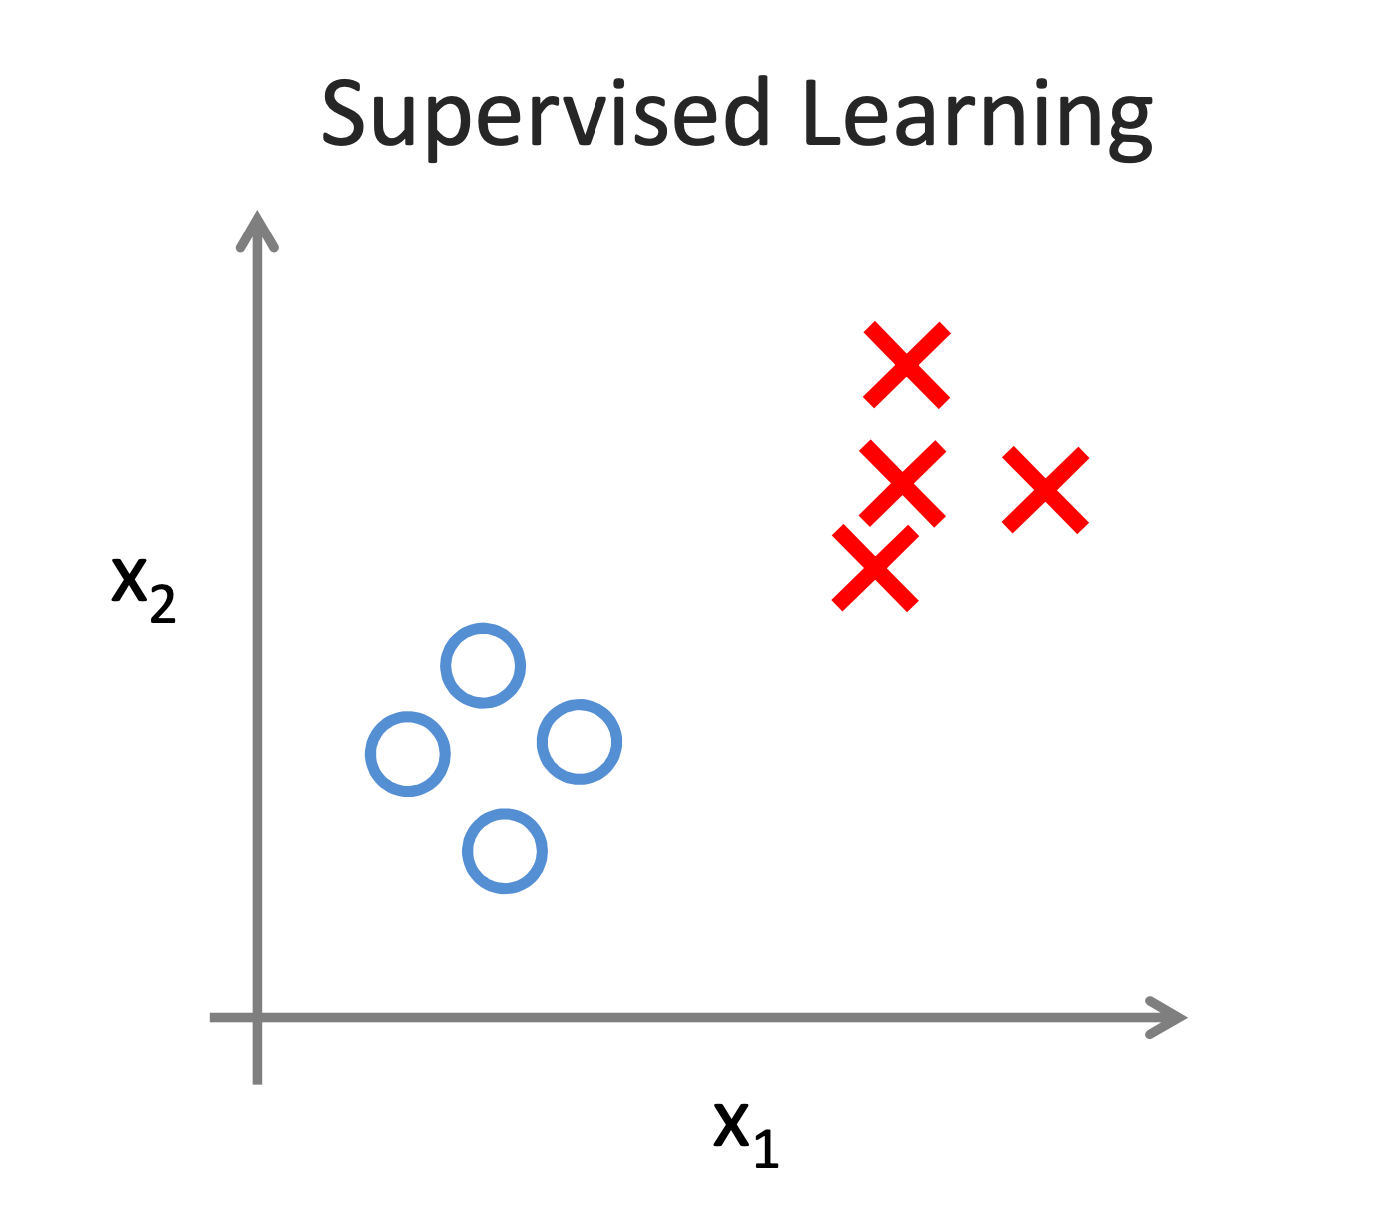
\includegraphics[width=0.5\textwidth]{image/supervised-learning.png}
        \caption{Supervised Learning}
        \label{fig:supervised-learning}
    \end{figure}

    \subsection{Unsupervised Learning}
    The right answer is not given, e.g. cocktail problem (distinguishing two voices from an audio file.)

    \begin{figure}[h]
        \centering
        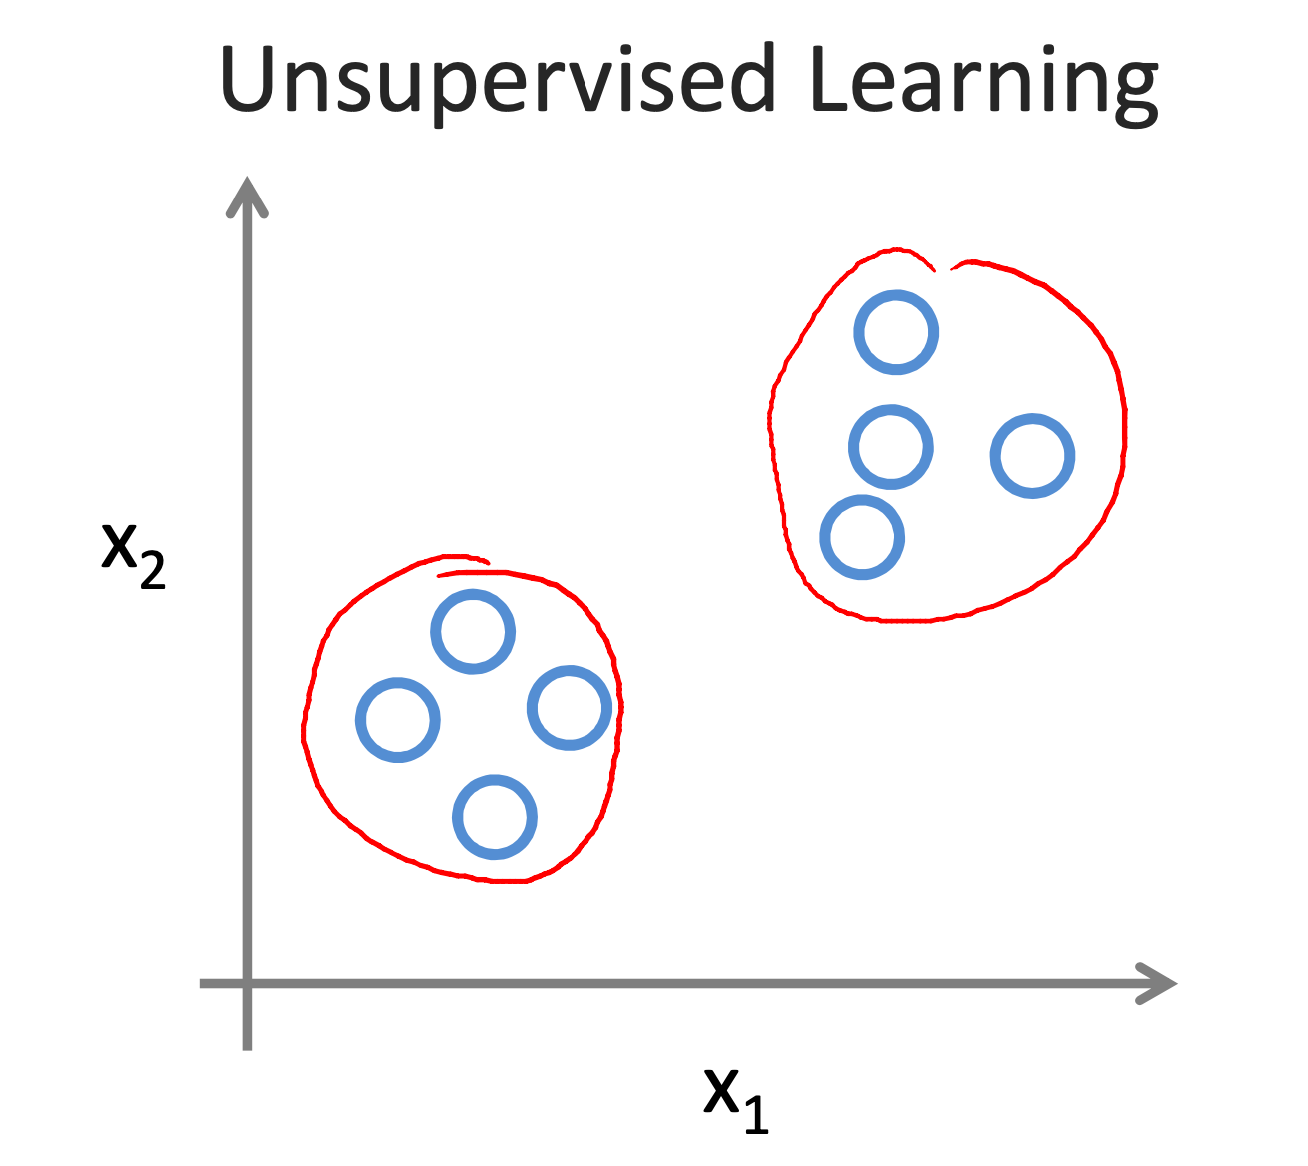
\includegraphics[width=0.5\textwidth]{image/unsupervised-learning.png}
        \caption{Unsupervised learning}
        \label{fig:unsupervised-learning}
    \end{figure}


    \section{Linear Regression with One Variable}
    \subsection{Model Representation}
        \subsubsection{Notations}
            For a training set:
           \begin{itemize}
               \item \textbf{m} = Number of training examples.
               \item \textbf{x} = ``input'' variable / features.
               \item \textbf{y} = ``output'' variables / ``target'' variable.
               \item \textbf{(x,y)} - one training example.
               \item \textbf{(x\textsuperscript{i},y\textsuperscript{i})} denotes the i\textsuperscript{th} training example 

           \end{itemize}

        \subsubsection{Hypothesis Function}
        
           A hypothesis function (h) maps input (x) to estimated output (y).
           How do we represent h?

           \begin{equation} 
               \boxed{ 
                   \textbf{Hypothesis Function}\hspace{10pt}  h_\theta (x) = \theta_0 + \theta_1x
           }
              \label{eq:hypothesis}
           \end{equation}

           We can apply \emph{Univariate linear regression} with respect to x. 
    \subsection{Cost Function}

    Recall \ref{eq:hypothesis}. The $\theta_i$s are parameters we have to choose. The intuition is is that we want to choose $\theta_i$ s such that h\textsubscript{$\theta$} is closest to y for our training examples (x,y).
    

      \begin{equation} 
          \boxed{ 
              \textbf{Cost Function}\hspace{10pt} J(\theta_0, \theta_1) = \frac{1}{2m} \sum_{i=1}^{m} (h_\theta(x^{(i)}) - y^{(i)} )^2
      }
          \label{eq:cost}
      \end{equation}
      

      \par \textbf{Summary} 
      \begin{enumerate}
          \item \textbf{Hypothesis  }$h_\theta (x) = \theta_0 + \theta_1x$
          \item \textbf{Parameters } $\theta_0, \theta_1$
          \item \textbf{Cost Function }$J(\theta_0, \theta_1) = \frac{1}{2m} \sum_{i=1}^{m} (h_\theta(x^{(i)}) - y^{(i)} )^2$
          \item \textbf{Goal } $\min_{\theta_0, \theta_1} J(\theta_0, \theta_1)$
    
      \end{enumerate}
        

          
   
    
    \subsection{Gradient Descent}
        \subsubsection{Intuition}
            \begin{enumerate}
                \item We have some function $J(\theta_0, \theta_1)$, we want to $\min_{\theta_0, \theta_1} J (\theta_0, \theta_1)$
                \item Outline: start with some $\theta_0, \theta_1$, keep changing  $\theta_0, \theta_1$ to reduce $J(\theta_0, \theta_1)$ until we end up at a minimum. 
            \end{enumerate}
        \subsubsection{Gradient Descent Algorithm}
            \textbf{Algorithm} \\
                repeat until convergence\{  
                    \[ \theta_j := \theta_j - \alpha \frac{\partial }{\partial \theta_j} J(\theta_0, \theta_1)\mbox{\hspace{10pt} (for j=0 and j=1)} 
                   .\] \}
        \\


           \textbf{Notes}
               \begin{enumerate}
                   \item the := denotes non-blocking assignment, i.e. simultaneously updates $\theta_0 and \theta_1$ 
                   \item We use the derivative to find a local minimum. 
                   \item $\alpha$ denotes the learning rate. Gradient descent can converge to a local minimum even when the learning rate $\alpha$ is fixed. As we approach a local minimum, gradient descent will automatically take smaller steps. Therefore it is not needed to decrease $\alpha$ over time. 
               \end{enumerate}

       \subsubsection{Gradient Descent with Linear Regression}
     
       Recall, we have:
       \begin{enumerate}
           \item Gradient Descent Algorithm: \\ 
               \linebreak
               repeat until convergence\{  
                    \[ \theta_j := \theta_j - \alpha \frac{\partial }{\partial \theta_j} J(\theta_0, \theta_1)\mbox{\hspace{10pt} (for j=0 and j=1)} 
                   .\] \}


           \item Linear Regression Model:
               \begin{center}
                   \[h_\theta (x) = \theta_0 + \theta_1x\]
                   \[J(\theta_0, \theta_1) = \frac{1}{2m} \sum_{i=1}^{m} (h_\theta(x^{(i)}) - y^{(i)} )^2\]             

               \end{center}

       \end{enumerate}
            
                 
                
    We can substitute the above equations, which gives us:
       \begin{center}
           \[\theta_0 := \theta_0 - \alpha \frac{1}{m} \sum_{i=1}^{m} (h_\theta(x^{(i)}) - y^{(i)} )\] 
               \[\theta_1 := \theta_1 - \alpha \frac{1}{m} \sum_{i=1}^{m} (h_\theta(x^{(i)}) - y^{(i)} ) \cdot x^{(i)}\]  

       
       \end{center} 
    


    \section{Review of Linear Algebra}

This is section is a basic review of linear algebra. I have skipped this section for now and will come back to it if time permits.

    \section{Linear Regression with Multiple Variables}

    \subsection{Multiple features}
    Recall in the single variable case, we have a single input (x), two parameters($\theta_0, \theta_1$). The hypothesis can be expressed as: \[
        h_\theta(x)= \theta_0 + \theta_1x
    .\] 
  
    Now, consider a generalized case where there are multiple features: X\textsubscript{1}, X\textsubscript{2}, X\textsubscript{3}. The information can be organized in a table with example numerical values:
    \begin{table}[htbp]
            \begin{center}
                 \begin{tabular}{||c c c c||} 
                 \hline
                  Sample Number (i) & X\textsubscript{1} &  X\textsubscript{2} & y \\ [0.5eX] 
                 \hline\hline
                 1 & 6 & 87837 & 787 \\ 
                 \hline
                 2 & 7 & 78 & 5415 \\
                 \hline
                 3 & 545 & 778 & 7507 \\
                 \hline
                 4 & 545 & 18744 & 7560 \\
                 \hline
                 5 & 88 & 788 & 6344 \\ [1ex] 
                 \hline
                \end{tabular}
             \caption{Sample Table}
             \label{tab:data}
         \end{center}
     \end{table}


        From Table \ref{tab:data}, one can see that each row is a sample a feature on each column.

    \subsubsection{Notation}

        \begin{enumerate}
            \item \textbf{n}: number of features.
            \item \textbf{x\textsuperscript{(i)}}: (row vector) input features of the i\textsuperscript{th} training example. i= 1, 2,\dots, m. 
            \item \textbf{x\textsuperscript{(i)}\textsubscript{j}}: value of feature j in the i\textsuperscript{th} training example. j= 1, 2, \dots, n.  

        \end{enumerate}

    \subsubsection{Hypothesis}

        Previously, 
        \[ 
        h_\theta(x)= \theta_0 + \theta_1\cdot x 
        \]
    

        Now, we can extend the hypothesis to :

        \[
            h_\theta(x) = \theta_0\cdot1 + \theta_1\cdot x_1 + \theta_2\cdot x_2  
        \]

        For convenience of notation, let's define x\textsubscript{0}=1, i.e. x\textsuperscript{i}\textsubscript{0}=1 $\forall$ i.

        Therefore, we have: \textbf{x}= $\left[ \begin{array}{c}
                                                    x_0 \\
                                                    x_1 \\
                                                    x_2 \\
                                                    \vdots \\
                                                    x_n
                                                 \end{array}
                                          \right]$
                                          and \textbf{$\theta$} = $\left[ \begin{array}{c}
                                                    \theta_0 \\
                                                    \theta_1 \\
                                                    \theta_2 \\
                                                    \vdots \\
                                                    \theta_n \\
                                                 \end{array}
                                          \right]$. 
        Then, the hypothesis function can be written as:

            \begin{equation}
                \begin{split}
                 h_\theta (x) &= \left[ \begin{array}{ccccc}
                                                \theta_0 & \theta_1 & \theta_2 & \dots & \theta_n 
        \end{array} 
                                    \right] \cdot \left[ \begin{array}{c}
                                                                x_0 \\
                                                                x_1 \\
                                                                x_2 \\
                                                                \vdots \\
                                                                x_n
                                                                 \end{array} \right] \\
                                                                 & = \theta^T\cdot \textbf{x}
            \end{split}
        \end{equation}
        

        This is \emph{Multivariate linear regression}.










    \subsection{Gradient Descent for Multiple Variables}
        \subsubsection{Algorithm}
            \textbf{Summary for Multivariables} 
                \begin{enumerate}
                    \item \textbf{Hypothesis  }$h_\theta (x) = \theta^T \cdot \textbf{x}$
                    \item \textbf{Parameters } $\mathbf{\theta}$
                    \item \textbf{Cost Function } $ J(\mathbf{\theta}) = \frac{1}{2m} \sum_{i=1}^{m} (h_\theta(x^{(i)}) - y^{(i)} )^2 $
                    \item \textbf{Goal } $ \min_{\mathbf{\theta}} J( \mathbf{\theta}) $
                \end{enumerate}

        
                \textbf{Gradient Descent for Multiple Variables}
                        repeat until convergence\{  
                            \[ \theta_j := \theta_j - \alpha \frac{\partial }{\partial \theta_j} J(\mathbf{\theta})\mbox{\hspace{10pt} (for j=0, 1,$\ldots$ n)}  
                            \] 
                        \}  \\


                        
                       \[\theta_j := \theta_j - \alpha \frac{1}{m} \sum_{i=1}^{m} (h_\theta(\mathbf{x^{(i)}}) - y^{(i)} ) \cdot x_j^{(i)}\] \\ 
                       
                       Note: $x_0^{(i)} = 1$, by definition.
        
         \subsubsection{Vectorized Implementation}

         One can work out the linear algebra and arrive at the following simplification using vectorized operations.
            The cost function $J$ can be expressed as:
            \begin{equation}
                J(\theta) = \frac{1}{2m} (\mathbf{X\theta} - \mathbf{y})^T (\mathbf{X\theta} - \mathbf{y} )
                \label{eq:vectorized-cost}
            \end{equation}
            
            The MATLAB implementation is as follows:
            \begin{lstlisting}
                m = length(y); % calculate how many samples 
                J = 1/(2*m)*((X*theta-y).')*(X*theta-y);

            \end{lstlisting}


            Gradient descent can be vectorized in the form:
            \begin{equation}
                \theta = \theta - \frac{\alpha}{m} \cdot \mathbf{X}^T \cdot (\mathbf{X\theta} - \mathbf{y}) 
                \label{eq:vectorized-gradient-descent}
            \end{equation}

            The MATLAB implementation is as follows:
            \begin{lstlisting}
                m = length(y); % number of training examples
                for iter = 1:num_iters
                    theta = theta - alpha/m* X.'*(X*theta -y);
            \end{lstlisting}


    \subsection{Gradient Descent in Practise I: Feature Scaling} 
    
        \begin{itemize}
            \item Idea: ensure each featurre are on a similar scale
            \item Get every feature into approx. $-1\leq x_i \leq1 $($\sim$ order)
            \item \textbf{Mean Normalization}: Replace $x_i$ with $\frac{x_i - \mu_i}{s_i}$, where $\mu_i$ and $s_i$ are the sample mean and standard deviation, respectively.

        \end{itemize}

    \subsection{Gradient Descent in Practise II: Learning Rate}
        
        \begin{itemize}
            \item Ensure gradient descent is working: plot $J_\theta$ over each number of iteration (not over $\theta$ !)
            \item Example automatic convergence test: for sufficiently small $\alpha$ $J_\theta$ should decrease by less than $10^{-3}$ i one iteration.
            \item If $\alpha$ is too small, gradient descent can be slow to converge.
            \item If $\alpha$ is too large, gradient descent may not converge.
            \item To choose $\alpha$, try 0.001, 0.003, 0.01, 0.03, 0.1, 0.3, 1\ldots (by 3x)
        \end{itemize}


    \subsection{Features and Polynomial Regression}
        We can fit into different polynomials by choice, using multivariate regression. Recall
        \[
            h_\theta (x) = \theta_0 + \theta_1x_1 + \theta_2x_2 +\theta_3x_3 
        \]  

        Let x\textsubscript{1} be x\textsuperscript{1}, x\textsubscript{2} be x\textsuperscript{2}, x\textsubscript{3} be x\textsuperscript{3}.
        Note we should still apply feature scaling to x\textsubscript{1}, x\textsubscript{2}, and x\textsubscript{3} individually! 


    \subsection{Normal Equation}

        The normal equation provides a method to solve for $\theta$ analytically. For our data with m samples, n features, recall each sample can be written as: 
       \[ 
        \mathbf{x^{(i)}} =  \begin{bmatrix}
            x_0^{(i)}\\
            x_1^{(i)} \\
            x_2^{(i)} \\
            \vdots \\
            x_j^{(i)}\\
           \vdots \\
           x_n^{(i)}
            \end{bmatrix}
        \]
        We can construct a design matrix:
        \[ \mathbf{X} = \begin{bmatrix}
            \horzbar & (x^{(1)})^T & \horzbar \\
            \horzbar & (x^{(2)})^T & \horzbar \\
            \horzbar & (x^{(3)})^T & \horzbar \\
                     & \vdots      &          \\
            \horzbar & (x_{m}^{T}  & \horzbar \\
         \end{bmatrix}
        \]

         Then $\theta$ can be found by the normal equation: 
                 \begin{equation}
                 \mathbf{\theta} = \mathbf{(X^TX)}^{-1}\mathbf{Ty}
                     \label{eq:normal}
                 \end{equation}

        
        Normal equation is useful as no $\alpha$ is required to and we do not need to iterate. However, we do have to compute $(X^TX)^{-1}$, which can be computationally expensive when n is large. The complexity is O($n^3$) for inverse operations. Gradient Descent is useful when n is large (many features). 

     \subsection{Normal Equation and Non-invertibility}

     What if $(X^TX)^{-1}$ is non-invertible? 

     \begin{itemize}
         \item Redundant features (linearly dependent), i.e. having same information in two different units.
         \item Too many features (i.e. m $\leq$ n). Delete some features or use regularization
     \end{itemize}




    \section{Octave/MATLAB Tutorial}

    \section{Logistic Regression}

    \subsection{Classification}
        
        \begin{itemize}
            \item Binary Classification: y $\in \{0, 1\}$, where 0 denotes the negative class; 1 denotes the positive class.
            \item Multi-class Classification:y $\in \{0, 1, \cdots, n\}$ 
        \end{itemize}

        We will be using binary classification: 
        \begin{itemize}
            \item Linear regression is not suitable for classification: since $h_\theta (x)$ can output out of range, i.e. $<0$ or $>1$. 
            \item We will use \textbf{logistic regression}, which ensures that the output $h_\theta (x)$ is between 0 and 1.
        \end{itemize}

    \subsection{Hypothesis Representation}

        \subsubsection{Logistic function}
            The idea is to have $ 0 \leq h_\theta (x) \leq 1$. Instead of the linear regression hypothesis: $h_\theta (x) = \theta^T x$, we will let:
                \[
                    h_\theta (x) = g (\theta^t x)
                ,\]

                where \[
                    g(z) = \frac{1}{1+e^{-z}}
                \]

                g(z) is known as the \textbf{logistic function}, also known as the Sigmoid function. Figure \ref{fig:sigmoid-function} shows a plot of the logistic function, which ranges from 0 to 1. 


                which yields 
                \begin{equation}
                    h_\theta (x) = \frac{1}{1+e^{-z}}
                    \label{eq:log-reg-hypo}
                \end{equation}


                \begin{figure}[htbp]
                    \centering
                    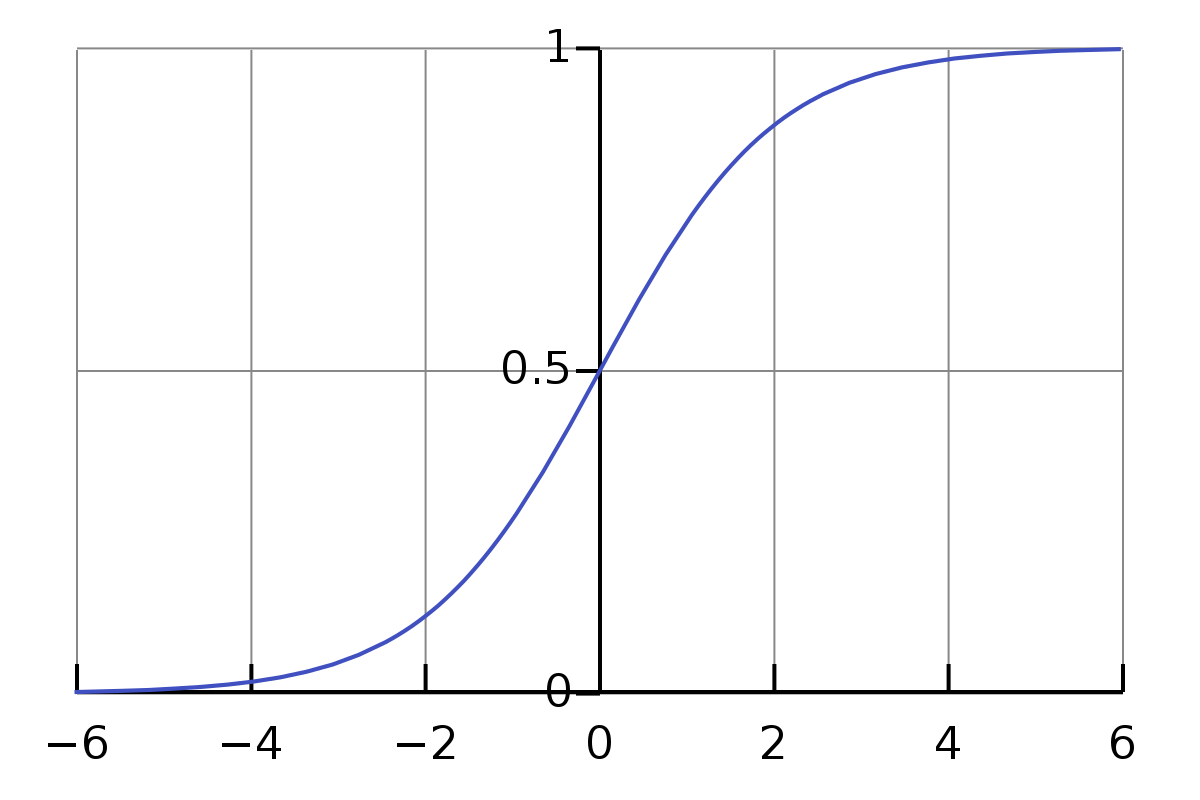
\includegraphics[width=0.5\textwidth]{image/sigmoid-function.png}
                    \caption{Sigmoid Function}
                    \label{fig:sigmoid-function}
                \end{figure}


        \subsubsection{Interpretation of Hypothesis Output}
        $ h_\theta (x)= $ estimated probability that y= 1 on input x. For example, $h_\theta(x)= 0.7$ gives us a probability of 70\% that are output is 1. 
        From a probability theory point of view, one can express $h_\theta (x)$ as $ P(y=1 \mid x;\theta)$. 

        Note that since this is a probability and the total probability sums up to 1, and the real y can only be either 0 or 1:
        \[
            P(y=0 \mid x; \theta) + P(y=1 \mid x;\theta) = 1
        \] 
            


    \subsection{Decision Boundary}

    Recall so far we have $h_\theta (x) = g(\theta^T x)$ and $g(z) = \frac{1}{1+exp(-z)}$. Suppose we set $h_\theta(x) = 0.5$ to be our determining factor for whether y= 0 or y =1. Note that from \ref{fig:sigmoid-function}, one can observe that $h_\theta(x) = 0.5$ corresponds to $\theta^T x = 0$, which is the \textbf{decision boundary}. The decision boundary is the equation which separates the different classes on a plot. There are linear and non-linear decision boundaries.


    \subsection{Cost function}

        Previously, we had $ J(\theta) = \frac{1}{m} \sum_{i=1}^{m} Cost( h_\theta ( x^{(i)}), y^{(i)} )$, where $Cost (h_\theta(x), y) = \frac{1}{2} (h_\theta(x) - y)^2$. 
        Now, the definition of the hypothesis $h_\theta$ has changed to $\frac{1}{1+exp(-\theta^T x}$, as a result the cost function is now non-convex. \\ 
        
            \textbf{Logistic Regression Cost Function}

            Therefore, a new cost function definition is needed. We propose: 

            \[
                Cost (h_\theta(x), y) = 
                \begin{cases}
                    -log(h_\theta(x))       &\quad \text{if } y=1 \\
                    -log(1- h_\theta(x))    &\quad \text{if } y=0 \\
                \end{cases}
            \] 

            Note that Cost=0, if y=1, $h_\theta(x) =1$; but as $h_\theta(x) \to 0$, then $Cost \to \infty$. This proposition captures the intuition that if $h_\theta(x)=0$, predict $P(y=1 \mid x;\theta)$, but y ends up being 1, we will penalize the learning algorithm by very large cost.
            
    \subsection{Simplified Cost Function and Gradient Descent}
        

            Since y can only be either 0 or 1, we can simplify the cost function.
       

            \begin{equation}
                \begin{split}
                    J(\theta)   &= \frac{1}{m}\, \sum_{i=1}^{m}\, Cost\,(\, h_\theta ( x^{(i)})\, ,\, y^{(i)} ) \\
                    &= \frac{-1}{m} \, [ \; \sum_{i=1}^{m}\, y^{(i)}\, log\, h_\theta (x^{(i)})\; +\; (1-y^{(i)})\: log\:(\,1-h_\theta(x^{(i)})\,) \;] 
                \end{split}
                \label{eq:simplified-logistic-cost-function}
            \end{equation}
            Equation \ref{eq:simplified-logistic-cost-function} is based on Maximum Likelihood Estimation.


            A vectorized implementation is, for a design matrix $\mathbf{X}$:
            \begin{equation}
                \boxed{
                    h = g(\mathbf{X\theta})
                }
                \label{eq:vectorized-logistic-hypothesis}
            \end{equation} 

            
            \begin{equation}
                \boxed{
                    J (\theta) = \frac{1}{m} (-y^T log(h) - (1-y)^T log(1-h) )
                }
                \label{eq:vectorized-logistic-cost-function}
            \end{equation} \\

            
            For gradient descent,we would want to $\min_{\theta} J(\theta)$:\\ 

             Repeat \{
                \[ 
                \theta_j := \theta_j - \alpha \frac{\partial }{\partial \theta_j} J(\theta)
                \]

            \} \\

   
            We can compute the partial derivative of $J(\theta)$, which is identical to that of linear regression:
            \[
                \frac{\partial }{\partial \theta_j} J(\theta) = \frac{1}{m} \sum_{i=1}^{m} ( h_\theta (x^{(i)}) - y^{(i)} )\cdot x^{(i)} 
            \]\\
            However, in this case the hypothesis function $h_\theta(x) = \frac{1}{1+exp(-\theta^T x}$ has changed!

            A vectorized implementation for this is:
            \begin{equation}
                \boxed{
                    \mathbf{\theta} := \mathbf{\theta} - \frac{\alpha}{m} \mathbf{X}^T( g (\mathbf{X\theta}) - \mathbf{y}))
                }
                \label{eq:vectorized-logistic-gradient-decent}
            \end{equation}



    \subsection{Advanced Optimization}
        \subsubsection{Taking a Step Back}
            If we take a step back, and consider essentially what tasks we are performing. We need to compute two things:
            \begin{enumerate}
                \item $J(\theta)$
                \item $\frac{\partial}{\partial \theta_j}J(\theta)$
            \end{enumerate}

        \subsubsection{Optimization Algorithm}
        There exists other more sophisticated and faster ways to optimize $\theta$ instead of gradient descent; they often do not involve selecting learning rate $\alpha$ and are more efficient. However, these algorithms are harder to code by hand. It is suggested that we use libraries for such algorithms. 

        We can write a single function that returns both  $J(\theta)$ (jVal) and  $\frac{\partial}{\partial \theta_j}J(\theta)$ (gradient):

        \begin{lstlisting}
        function [jVal, gradient] = costFunction(theta)
            jVal = [...code to compute J(theta)...];
            gradient = [...code to compute derivative of J(theta)...];
        end
            
        \end{lstlisting}

        Then we can use octave's "fminunc()" optimization algorithm along with the "optimset()" function that creates an object containing the options we want to send to "fminunc()".

        \begin{lstlisting}
            options = optimset('GradObj', 'on', 'MaxIter', 100);
            initialTheta = zeros(2,1);
            [optTheta, functionVal, exitFlag] = fminunc(@costFunction, initialTheta, options);
            
        \end{lstlisting}
        

        We then give to the function "fminunc()" our cost function, our initial vector of theta values, and the "options" object that we created beforehand.
        \subsection{Multiclass Classification: One-vs-All}
            Now, let's extend the binary classification of data to multi-classes, i.e expanding our definition of y s.t. y=\{0, 1, \ldots, n\}.
            We will divide out problem into n+1 (0\ldots n) binary classification problems. In each problem, we predict the probability that y is a memember of one of our class. We train a logistic regression classifier $h_\theta ^{(i)} (x) $ $\forall$ i to predict y = i:
            \begin{equation}
                h_\theta^{(i)} (x) = P (y=i \mid x;\theta)
                \label{eq:multiclass-logistic-classifier}
            \end{equation}

            Figure \ref{fig:multi-class-regression} shows an example of the procedure of classifying three classes. We choose one class and then lump all the others into a single second class (hence the name One-vs-All). We apply the binary logisic regression repeatedly and use the hypothesis that returns the highest value. 

            \begin{equation}
                prediction\,=\: \max_{i}\: (\, h_\theta ^{(i)} (x) \,)   
                \label{eq:max-log-regre}
            \end{equation}
            

            \begin{figure}[htbp]
                \centering
                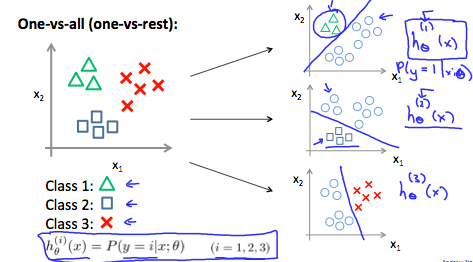
\includegraphics[width=\textwidth]{image/multi-class.png}
                \caption{Example of Multiclass Logistic Regression}
                \label{fig:multi-class-regression}
            \end{figure}

    \section{Regularization}
    \subsection{The problem of overfitting}
    There are two types of errors in fitting functions to data, in which data shows the structure is not captured by the model. The terminology applies to both linear and logistic regression. Figure \ref{fig:fitting} shows an example of each fitting case. 

            \begin{enumerate}
                \item Underfitting (high bias): when the form of our hypothesis function ($h_\theta (x)$) maps poorly to the trend of data. It is usually caused by a function that is either too simple or uses too little features. 
                \item Overfitting (high variance): when hypothesis function learns the training set very well hence fits the available data but does not generalize well to predict new data, i.e fitting too many details. It is usually caused by a complicated function that creates a lot of unneccessary curves and angles unrelated to the data. 
            \end{enumerate}
        
            \begin{figure}[htbp]
                \centering
                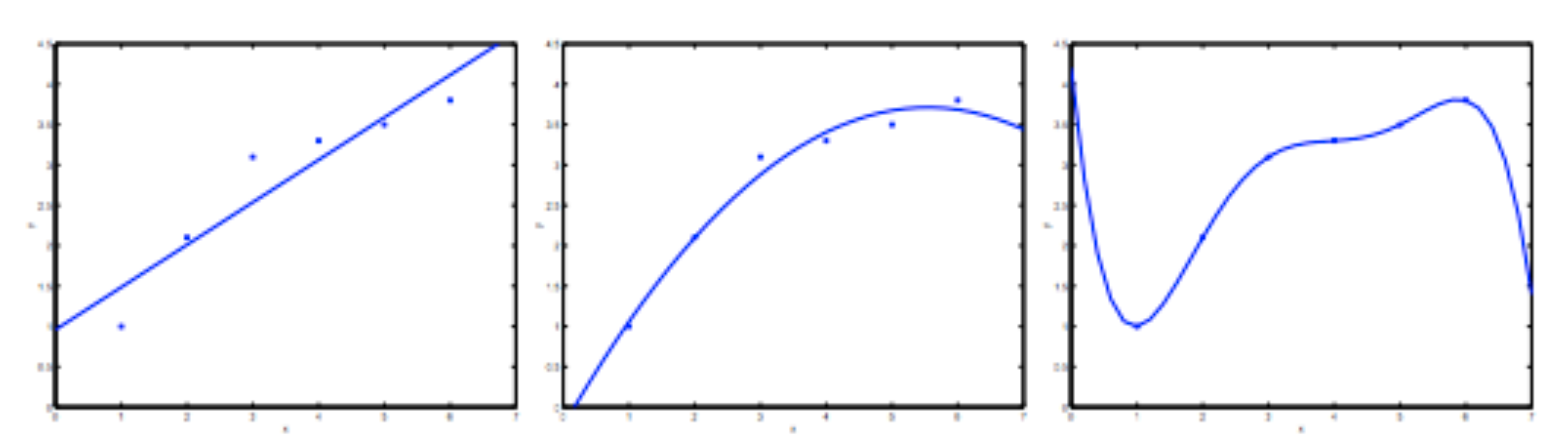
\includegraphics[width=\textwidth]{image/fitting.png}
                \caption{Three scenarios of fitting: underfit(left), good fit (middle), and overfit(right).}
                \label{fig:fitting}
            \end{figure}

        There are two main options to address the issue of overfitting:
            \begin{enumerate}
                \item Reduce the number of features
                    \begin{itemize}
                        \item manually select which features to keep.
                        \item Use a model selection algorithm (later in the course).
                    \end{itemize}
                \item \textbf{Regularization}
                    \begin{itemize}
                        \item Keep all the features, but reduce the magnitude of parameters $\theta_j$
                        \item Regularization worls well when we have a lot of slightly useful features. (Each contributes a bit to predict y)
                    \end{itemize}
            \end{enumerate}


    \subsection{Cost Function}
        \subsubsection{Intuition}
            Suppose we have overfitting, we can reduce the weight that some of the terms in our function carry by penalizing the feature parameter with increased cost. Consider the following hypothesis function : \[
            \theta_0 + \theta_1 x + \theta_2 x^2 + \theta x^3 + \theta x^4
        .\] We would want to make the function more quadratic, which means we would like to reduce the influence of $\theta_3$ and $\theta_4$. Since our goal was to minimize the cost function $J(\theta)$, we could modify the original cost function \[
            \min_\theta \frac{1}{2m} \sum_{i=1}^{m} ( h_\theta (x^{(i)}) - y^{(i)} )^2 + 1000\cdot \theta_3^2 + 1000\cdot \theta_4^2
        .\] This will force $\theta_3$ and $\theta_4$ to be close to zero, and make the original hypothesis function more quadratic.

        \subsubsection{Regularization}
            Now, we can take a step further and regularize all theta parameters: 

            \begin{equation}
                \min_\theta \:\:[ \frac{1}{2m} \sum_{i=1}^{m} ( h_\theta (x^{(i)}) - y^{(i)} )^2 ] + \lambda \sum_{j=1}^{n} \theta_j^2
                \label{eq:regularization-general-form}
            \end{equation}

            Here we are performing two separate operations which can be oberved as the two terms in Equation \ref{eq:regularization-general-form}. The first term corresponds to ``training the data'', and the second term relates to ``keeping the parameters small''. The coefficient $\lambda$ is the \textbf{regularization parameter} and determines the balance between the aforementioned two objectives. Note that if $\lambda$ is too big ($\approx$ 10\textsuperscript{10}), then all $\theta_j \approx 0$, except for $\theta_0$ (the constant term). This makes $h_\theta \approx 0$ and defies the purpose of training and leads to underfitting ( a flat horizontal line).




    \subsection{Regularized Linear Regression}
    \subsubsection{Gradient Descent} 
        We will modify the gradient descent function to separate out $\theta_0$ from the rest of the parameters because we do not want to penalize $\theta_0$.\\

        repeat until convergence\{  
            \[ \theta_0 := \theta_0 - \alpha \frac{1}{m} \sum_{i=1}^{m} ( h_\theta (x^{(i)}) - y^{(i)}) x_0^{(i)}\] 

            \[
                \theta_j := \theta_j - \alpha [ ( \frac{1}{m} \sum_{i=1}^{m} ( h_\theta (x^{(i)}) - y^{(i)}) x_j^{(i)} ) + \frac{\lambda}{m}\theta_j]
            \] 

        \} , where $j\in \{1, 2, \ldots, n\}$ \\

        The above equation can be re-arranged to get the final form:

        \begin{equation}
            \boxed{
            \theta_j := \theta_j (1-\alpha \frac{\lambda}{m}) - \frac{\alpha}{m} \sum_{i=1}^{m} ( h_\theta (x^{(i)}) - y^{(i)}) x_j^{(i)}
        }
            \label{eq:regularized-gradient-descent}
        \end{equation}

        The term $(1-\alpha \frac{\lambda}{m})$ will always be less than 1. Intuitively, this reduces the parameter, then the rest of equation \ref{eq:regularized-gradient-descent} carries the normal gradient descent.
        
        \subsubsection{Normal Equation}

        Recall from our previous normal equation (Equation \ref{eq:normal}), we have the design matrix \textbf{X} such that
            \[
            \mathbf{X} = \begin{bmatrix}
                \horzbar & (x^{(1)})^T & \horzbar \\
                \horzbar & (x^{(2)})^T & \horzbar \\
                \horzbar & (x^{(3)})^T & \horzbar \\
                         & \vdots      &          \\
                \horzbar & (x_{m}^{T}  & \horzbar \\
             \end{bmatrix}
            \]

            Now, to add in regularization to Equation \ref{eq:normal}, we get:

                 \begin{equation}
                     \boxed{
                     \mathbf{\theta} = (\mathbf{(X^TX)}+ \lambda\cdot\mathbf{L})^{-1} \mathbf{x}^Ty
                    }
                     \label{eq:regularized-normal}
                 \end{equation}

                 where $ L \in \mathbb{R}^{(n+1) \times (n+1)}$ 

                \begin{equation}
                    L = \begin{bmatrix}
                            0 & & & \\
                            & 1 & & \\
                            & &  \ddots & & \\
                            & &  & \ddots & \\
                            & & & & & 1 
                        \end{bmatrix}
                    \label{eq:regularized-L}
                \end{equation}
                
                Supopose non-invertibility arises: $m \leq n$, i.e \#examples is less than or equal to number of features, then using a $\lambda > 0$ in Equation \ref{eq:regularized-normal} will resolve the non-invertibility.



    \subsection{Regularized Logistic Regression}
            
        \subsubsection{Regularized Logistic Cost Function}
        We can modify our old logistic cost function (Equation \ref{eq:simplified-logistic-cost-function}) to apply regularization. 
                    \begin{equation}
                        \boxed{
                        J(\theta) = \frac{-1}{m} \, \sum_{i=1}^{m}\, [ y^{(i)}\, log\, h_\theta (x^{(i)})\; +\; (1-y^{(i)})\: log\:(\,1-h_\theta(x^{(i)})\,) ] + \frac{\lambda}{2m} \sum_{j=1}^{n} \theta_j^2
                    }
                        \label{eq:logistic-cost-function-regularized}
                    \end{equation}
                    Note that the second sum in Equation \ref{eq:logistic-cost-function-regularized} explicitly exludes the bias term $\theta_0$. 



        \subsubsection{Regularized Logistic Gradient Descent}
            The gradient descent is similar to that of linear regression; however note that the hypothesis function has been updated to Equation \ref{eq:log-reg-hypo}.\\

               repeat until convergence\{  
            \[ \theta_0 := \theta_0 - \alpha \frac{1}{m} \sum_{i=1}^{m} ( h_\theta (x^{(i)}) - y^{(i)}) x_0^{(i)}\] 

            \[
                \theta_j := \theta_j - \alpha [ ( \frac{1}{m} \sum_{i=1}^{m} ( h_\theta (x^{(i)}) - y^{(i)}) x_j^{(i)} ) + \frac{\lambda}{m}\theta_j]
            \] 

        \}






\end{document}


